



  In the following diagram, what is the length of $\overline{AC}$?
\begin{center}
 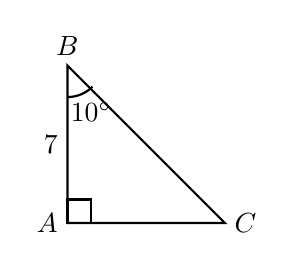
\begin{tikzpicture}
 
 \draw (0,0) --(2,0)--(0,2)--cycle  [thick,-,>=latex];
 \draw (0,0) --(0,.3)--(.3,.3)--(.3,0)--cycle  [thick,-,>=latex];
\draw[thick] (0,1.60) arc (270:315:.45);

  \draw node[below] at (.3,1.65) {$10^\circ$};
  \draw node[left] at (0,0) {$A$};
   \draw node[above] at (0,2) {$B$};
      \draw node[right] at (2,0) {$C$};
            \draw node[left] at (0,1) {$7$};
      
\end{tikzpicture}
\end{center}



\ifsat
	\begin{enumerate}[label=\Alph*)]
		\item    $\frac{\tan(10^\circ)}{7}$
		\item  $7\tan(10^\circ)$ %
		\item $\frac{7}{\sin(10^\circ)}$ 
		\item $7\cos(10^\circ)$
	\end{enumerate}
\else
\fi

\ifacteven
	\begin{enumerate}[label=\textbf{\Alph*.},itemsep=\fill,align=left]
		\setcounter{enumii}{5}
		\item    $\frac{\tan(10^\circ)}{7}$
		\item  $7\tan(10^\circ)$ %
		\item $\frac{\cos(10^\circ)}{7}$
		\addtocounter{enumii}{1}
		\item $\frac{7}{\sin(10^\circ)}$ 
		\item $7\cos(10^\circ)$
	\end{enumerate}
\else
\fi

\ifactodd
	\begin{enumerate}[label=\textbf{\Alph*.},itemsep=\fill,align=left]
		\item    $\frac{\tan(10^\circ)}{7}$
		\item  $7\tan(10^\circ)$ %
		\item $\frac{\cos(10^\circ)}{7}$
		\item $\frac{7}{\sin(10^\circ)}$ 
		\item $7\cos(10^\circ)$
	\end{enumerate}
\else
\fi

\ifgridin
  $7\tan(10^\circ)$ %
		
\else
\fi

